\documentclass{article}
\usepackage[spanish]{babel}
\usepackage[numbers,sort&compress]{natbib}
\usepackage{graphicx}
\usepackage{subfigure}
\usepackage{url}
\usepackage{hyperref}
\usepackage{amsmath}
\usepackage[top=15mm, bottom=40mm, left=15mm, right=15mm]{geometry}
\setlength{\parskip}{2mm}
\setlength{\parindent}{0pt}
\usepackage{listings}



\author{3175}
\title{Diagramas de Voronoi}
\date{\today}

\begin{document}

\maketitle


\section{Introducción}

También llamados planos de Thiessen, son una forma geométrica que permite construir una partición del plano euclídeo. Son llamados diagramas de Voronoi pues fueron estudiados por el matemático ruso Gueurgi Voronói en 1907 \cite{ref1}.
 
\section{Objetivo}
Evaluar si el tamaño de la zona de la matriz y la cantidad de semillas iniciales realizando variaciones de éstos factores determina el tamaño de una grieta que se propaga con una preferencia por los limites de los clusters en la zona.

\section{Metodología}
Se inicia con el código proporcionado en la práctica 4 \cite{elisawebp4} para la generación del diagrama de voronoi y el modelo de propagación de la grieta. Posteriormente se realizaron iteraciones con variaciones de n=zona (30, 50, 70) y k=número de semillas iniciales (10, 12, 14, 16). Se definieron 200 repeticiones para que la muestra sea representativa y se evaluó en base a longitud que la grieta presentada. Finalmente se realiza un análisis ANOVA de dos factores a los datos para determinar si la varianza de los datos entre los tratamientos es significativa. 

\section{Resultados}
En los resultados representados en la gráfica 1 se puede observar que los promedios de la longitud de las grietas son cercanos entre los distintos tipos de tratamientos, sin embargo, se observa un tendencia ascendente en los máximos cuando el número de semillas aumenta así como el tamaño de la zona.

\begin{figure}[hbtp]
\centering
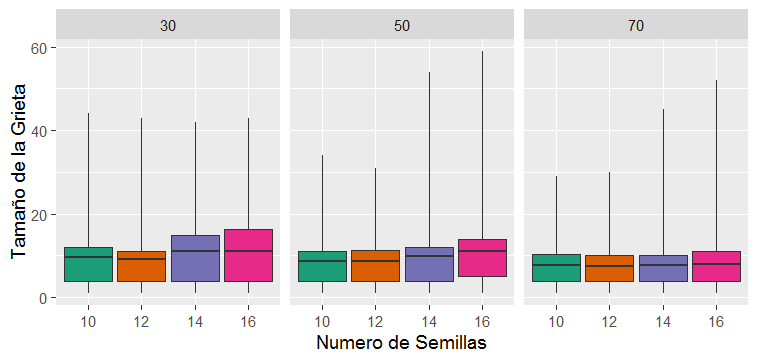
\includegraphics[width=10cm]{P4_grieta.png}
\caption{Gráfica de largos de grieta alternando en los diferentes tratamientos de tamaño de zona y cantidad de semillas iniciales}
\end{figure}

Se realizaron las hipótesis nulas en donde: "El tamaño de zona no determina el tamaño de la grieta formada", "El número desemillas no determina el tamaño de la grieta formada" y la relación entre los dos factores "El tamaño de la zona y de la semilla en conjunto no determina el tamaño de la grieta".

\begin{lstlisting}

                    Df Sum Sq Mean Sq F value   Pr(>F)    
TZonas              2   2657  1328.5  24.228 3.83e-11 
Tsemillas           3   1011   336.9   6.144  0.00037 
TZonas:Tsemillas    6    411    68.5   1.249  0.27794   
Residuals        2388 130939    54.8   
\end{lstlisting}

Debido a los resultados del análisis ANOVA se pueden descartar las hipótesis nulas de los tratamientos, sin embargo, se acepta la hipótesis nula en la que la variación de el tamaño de zona y la cantidad de semillas no influye en el tamaño de la grieta con una probabilidad de 27.7%.


\section{Conclusiones}
Se puede concluir en base a los resultados que los tamaños de las grietas si están influenciadas predominantemente por el tamaño de las zonas y en cierta medida por la cantidad de semillas, debido a que ambas variables determinan el medio en dimensiones y configuración respectivamente por el cual la grieta se propaga. Adicionalmente, no hay variación significativa en los resultados entre las iteraciones de las combinaciones de tratamientos, se puede observar que los promedios de los longitudes de las grietas están muy cercanos entre si.









\bibliographystyle{plainnat}
\bibliography{biblio4}
\end{document}